    
\documentclass[11pt]{article}
\usepackage{times}
\usepackage{fullpage, graphicx}
\usepackage{enumitem}
\usepackage[colorlinks=true, allcolors=blue]{hyperref}

\title{Automatic Illustration of Text via Multimodal Interaction}
\author{Stergious Aji - 2546916A}

\begin{document}
\maketitle

\section{Status report}

\subsection{Proposal}\label{proposal}
\subsubsection{Motivation}\label{motivation}
Video production is a very time consuming process and many parts of it can be easily automated like the making of illustrated music lyric videos, educational content or podcasts. This can greatly improve accessibility, not to mention, provide better mediums for teaching and learning. An automatic videographic tool would aim to sequence relevant images, that are based on the textual content present in the audio, in a timely manner. However, at the moment, there lacks a generally accepted, objective procedure at evaluating the results of such a system. User surveys can provide widely subjective and differing opinions on the relevancy of the images and their timeliness. Additionally, each time the system is changed, new user surveys must be conducted to re-evaluate it. For this reason, the system's output should be gauged against an immutable ground truth which would yield standardised metrics and can therefore be compared and repeated.


\subsubsection{Aims}\label{aims}
The aims of this project will be to develop a software framework to make user corroborated ground truths of automated videographic content. The user will have to select images that they believe are most relevant to the given audio chunks, out of a set that the system retrieves. This can then be objectively and systematically evaluated against other automated videography systems on the same audio sources. This evaluation aims to provide standardised performance metrics for any general automated videography tool.


\subsection{Progress}\label{progress}
\begin{itemize}[noitemsep]
    \item Language and Web framework chosen: System will be built using Python and the Django Web Framework.
    \item Main videography generation pipeline implemented with pytube API to take YouTube URLs as input.
    \item Pipeline made more automated by using Shazam API to recognise songs and artist names and MusixMatch API to retrieve its corresponding synced lyrics.
    \item Dataset to retrieve text and images from selected: Wikipedia-based Image-Text dataset (WIT).
    \item Background research conducted on solely text indexing and querying.
    \item Text indexing and querying implemented using PyTerrier.
    \item Background research conducted on solely image vectorising using its Wikipedia caption.
    \item Started development of the prototype Django Web Application.
\end{itemize}


\subsection{Problems and risks}\label{problems-and-risks}
\subsubsection{Problems}\label{problems}
\begin{itemize}[noitemsep]
    \item Initial compatibility issues experienced with the JDK version used by PyTerrier and the one installed in my computer. Luckily once problem was identified, it was easily fixed.
    \item Researching an efficient way of indexing images and text in a multimodal space. Currently researching into CLIP to solve problem.
    \item Implemented Shazam API is not fully robust as in very rare cases, it fails to recognise well-known songs. This can be solved by running the search again, although, need to look into a better solution.
    \item Need to find a way to systematically download the images from the WIT dataset which currently only contain image URLs.
    \item Solely using text to index and query images do not provide very relevant images. Need to experiment with more vectorisers as currently I am only using TF-IDF.
\end{itemize}


\subsubsection{Risks}\label{risks}
\begin{itemize}[noitemsep]
    \item Sufficient space is needed to store the static collection of images from the large WIT dataset. \\
    \textbf{Mitigation:} Systematically collect a subset of images as there are many that can be considered useless for this application.
    \item The system pipeline still relies on external APIs to download videos, recognise songs and retrieve synced lyrical data which can hinder the system if any one fails. \\
    \textbf{Mitigation:} Instead of retrieving audio from downloaded YouTube videos, an option to upload MP3 files should be implemented as well.
    \item At the moment, it is not clear how the evaluation metrics will be calculated. No clear mitigation currently but will be looked into, in the future.
\end{itemize}

\subsection{Plan}\label{plan}
The following Gantt Chart in Figure \ref{fig:gantt_chart} shows my plan to develop the software for my project during the Winter weeks. This work will then continue through Semester 2 and the deliverables are outlined below. 

\noindent \textbf{Winter}
\begin{figure}[h!]
    \centering
    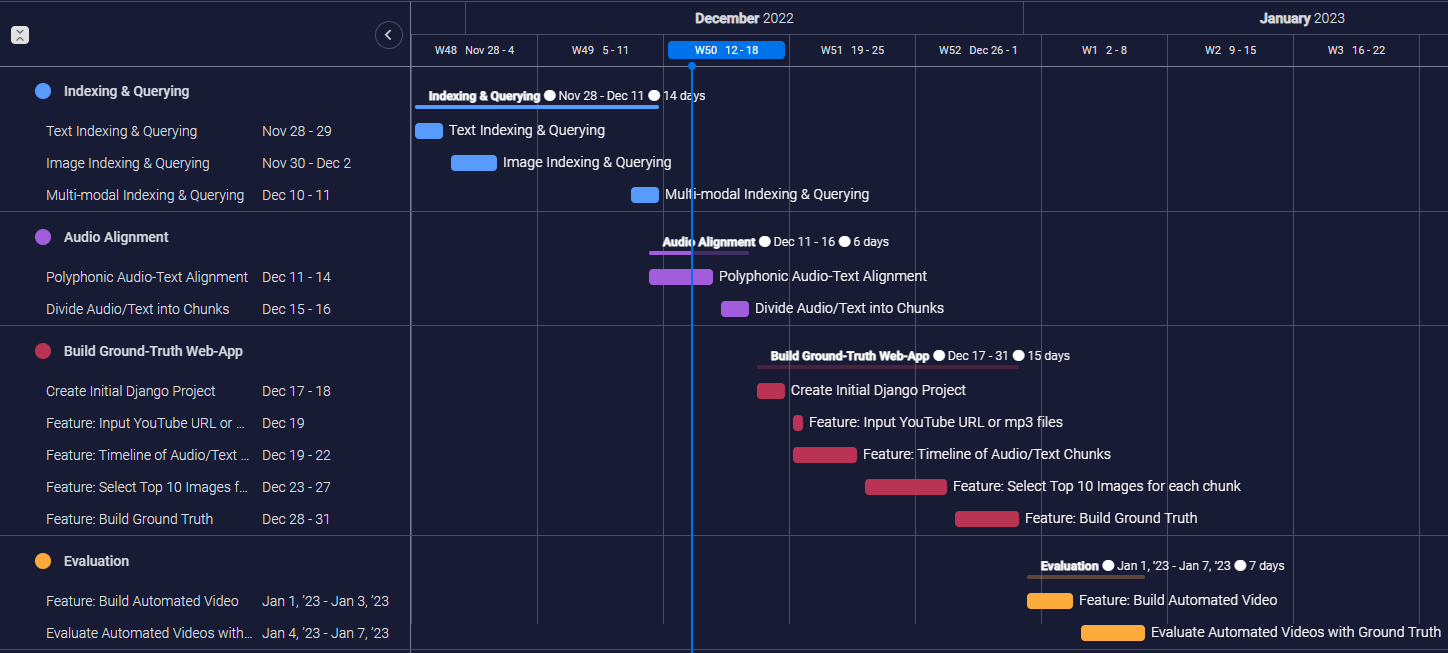
\includegraphics[scale=0.34441]{project-gantt-chart.png}
    \caption{Project Development Gantt Chart}
    \label{fig:gantt_chart}
\end{figure}
\\

\noindent \textbf{Semester 2}

\noindent
\begin{itemize}[noitemsep]
    \item Weeks 1-2: Polish web solution to function for input MP3 files and YouTube URLs.
    \begin{itemize}
        \item \textbf{Deliverable:} Working web application that outputs generated videograpy data for inputted audio sources.
    \end{itemize}
    \item Weeks 3-5: Create ground truth data on previously agreed songs.
    \begin{itemize}
        \item \textbf{Deliverable:} Ground truth data for the selected songs.
    \end{itemize}
    \item Weeks 6-8: Research and work on calculating performance metrics of automated videography tool.
    \begin{itemize}
        \item \textbf{Deliverable:} Performance metrics for the generic automated videographic tool for the selected songs using the ground truths.
    \end{itemize}
    \item Weeks 8-10: Write up of dissertation.
    \begin{itemize}
        \item \textbf{Deliverable:} First draft submitted to supervisor.
    \end{itemize}
\end{itemize}
\end{document}